\chapter{Dynamics of Rigid Bodies}
\label{chapter:dynamics}

While \textbf{kinematics} describes the motion of any object mathematically,
\textbf{dynamics} describes \emph{what} causes motion to change


\section{Laws of Motion}

\subsection{First Law of Motion}

The first law of motion, called the \emph{law of equilibrium}, describes what
happens when there are no forces act on an object:

\begin{definition}
  \textbf{First Law:} An object will remain in its state of rest or uniform
    motion, until a net external force is applied to it.\footnote{Lex I:
  Corpus omne perseverare in statu suo quiescendi vel movendi uniformiter
  in directum, nisi quatenus a viribus impressis cogitur statum illum
  mutare.}
\end{definition}
The first law, called the \emph{law of inertia}, states that when the sum
of all the forces acting on an object is balanced, In other words, the three
equations below are equivalent:
\begin{important-equation}
  \bm F_\text{net}=\sum\bm F=\bm 0
  \quad\longleftrightarrow\quad
  \bm v=\text{constant}
  \quad\longleftrightarrow\quad
  \bm a=\bm 0
\end{important-equation}

What is not stated explicitly by Newton is that the first law of motion is only
valid when the mass of the object is constant. In other words, the first law of
motion, as stated above, will \emph{not} work for:
\begin{itemize}[itemsep=3pt]
\item A rocket expelling spent fuel as it is launched towards space
\item A train car collecting grain though its open top
\end{itemize}
In Chapter~\ref{chapter:momentum}, we will modify the first law of motion
to include objects with changing mass. In Chapter~\ref{chapter:cm}, we will
examine the law's relationship to an object's centre of mass.

When the net force on an object is zero ($\sum\bm F=\bm 0$) then the
object is in a \emph{state of translational equilibrium}. Equilibrium can be
either:
\begin{itemize}[nosep,leftmargin=12pt]
\item\textbf{dynamic equilibrium} when the object is moving relative to the
  observer), or
\item\textbf{static equilibrium}, when the object is not moving relative to the
  observer
\end{itemize}

%\item Common examples:
%  \begin{itemize}
%  \item A hockey puck sliding on very smooth ice has gravity and normal
%    force, but the net force is zero
%  \item A car traveling on a highway at \SI{100}{\kilo\metre\per\hour}
%    has many forces acting on it, but the net force is zero 
%  \end{itemize}
%\item{\color{red!80!black}This is a special case that assumes a constant
%  mass}
%\end{itemize}

%\subsubsection{Aristotle: The Wrong Interpretation}
Prior to Galileo, the understanding of motion came primarily from Greek
philosopher Aristotle, who said that any body in motion will come its natural
state: at rest. Aristotle's idea ``makes sense'' from everyday experience. For
example: slide a book across a table, it will eventually stop. However, Galileo
pointed out that Aristotle's philosophy is ambiguous: absolute rest cannot be
determined because all motion is relative.

\textbf{Absolute rest cannot be determined:} Objects that are stationary in one
coordinate system can be moving relative to another (see
Section~\ref{sec:relative-motion}). A cup of water, shown in Fig.~\ref{fig:cup},
is on the tray table on an airplane in flight. The cup is stationary relative
to the passengers, but moving relative to anyone outside watching the airplane
fly by.
\begin{figure}[ht]
  \centering
  \pic{.4}{dynamics-calculus/coffeecup}
  \caption{A cup of water on an airplane is flight is stationary only
    passengers on the airplane, but not to observers outside}
  \label{fig:cup}
\end{figure}

\textbf{Uniform motion is indistinguishable from rest:} If I drop a tennis ball
while standing on the ground (Fig~\ref{fig:tennisball}), the ball falls
straight down with an acceleration due to gravity. If I repeat this while on an
airplane travelling in uniform motion (i.e.\ constant velocity) in the air, I
will observe exactly the same thing. The motion of the ball gives me no
information about whether I am at rest on in uniform motion
\begin{figure}[ht]
  \centering
  \pic{.4}{dynamics-calculus/Aging-Self-2}
  \caption{Observing the motion of a dropped tennis ball gives no hint as to
    whether you are stationary or moving in uniform motion.}
  \label{fig:tennisball}
\end{figure}



\subsection{Second Law of Motion}
\label{sec:2nd-law-of-motion}

The secon law of motion addresses what happens when the forces acting on an
object is not balance, i.e.\ when the net force is not zero.

\begin{definition}
  \textbf{Second Law:} The acceleration of an object is proportional to, and
  along the direction of, the net external force.\footnote{Lex II: Mutationem
  motus proportionalem esse vi motrici impressae, et fieri secundum lineam
  rectam qua vis illa imprimitur.}
\end{definition}
The second law states that the acceleration of an object is the direct result
of the imbalance of forces, and that the relationship is \emph{linear} (i.e.\
when the net force is double, the acceleration also doubles). The first two
laws of motion can be summarized by perhaps one of the most important and
recognizable equations in physics:
\begin{important-equation}
  \bm F_\text{net}=m\bm a
\end{important-equation}
The \emph{proportionality} between the net force and the acceleration of the
object is its mass. In fact, mass is defined as the ratio between the magnitude
of the net force acting on an object and the magnitude of the resultant
acceleration:
\begin{important-equation}
  m=\frac{|\bm F_\text{net}|}{|\bm a|}
\end{important-equation}
As such, mass is an intrinsic property of an object, and the same net force on
the object will \emph{always} result in the same acceleration, regardless of
what the net force is composed of, and whether the object is on Earth, on the
Moon, or in deep space.

Both the first and second laws of moton, as stated by Newton, require that the
mass of the object be constant. For non-constant mass, net force is the rate of
change of momentum $\bm p$.
\begin{equation*}
  \bm F_\text{net}(t)=\diff{\bm p}t
\end{equation*}
The topic of momentum will be studied in detail in
Chapter~\ref{chapter:momentum}.
%Like the first law, the second law of motion as descrribed by Newton is also a
%``special case'' that assumes a constant mass. We can summarize the first two
%laws into one of the most recognizable equation:
%\begin{important-equation}
%  \bm F_\text{net}(t)=\sum\bm F=m\bm a(t)
%\end{important-equation}

%
%
%\subsection{Defining Mass}
%What is \textbf{mass} then? It is
%\begin{itemize}
%\item the property of an object that relates its acceleration to the force
%  applied to it. Literally, it means:
%  \begin{equation}
%    m\equiv\frac{F_\text{net}}a
%  \end{equation}
%\item Intrinsic to the object itself
%\item This is explicitly referred to as the object's \textbf{inertial mass}
%\end{itemize}




\subsection{Third Law of Motion}
\label{sec:3rd-law}
The third law of motion deals with the interaction between objects when forces
are created, and how objects apply forces on each other:
\begin{definition}
  \textbf{Third Law:} To every action there is always opposite and equal
  reaction; the mutual actions of two bodies upon each other are always
  equal, and directed to contrary parts.
\end{definition}
Mathematically, we can write that the force object $A$ exerts on bbject $B$
($\bm F_{AB}$, the action force) is equal in magnitude but opposite in
direction to the force that object $B$ exerts on object $A$ ($\bm F_{BA}$, the
reaction force).
\begin{important-equation}
  \bm F_\text{AB} = -\bm F_\text{BA}
  \label{eq:third-law}
\end{important-equation}
The negative sign in Eq.~\ref{eq:third-law} indicates that the forces are in
opposite direction. It must be noted that
\textbf{the action and reaction forces must act on \emph{different} objects}.

The implication of the third law of motion is that forces are always created in
pairs: it is impossible for one object to exert a force on another without also
simultaneously being acted on by the other object. In
Chapter~\ref{chapter:energy}, we will show that the third law of motion is
crucial in formulating (and understanding) the law of conservation of energy.
In Chapters~\ref{chapter:momentum} and ~\ref{chapter:cm}, we will show that the
third law of motion is, in fact, an application of the first law of motion,
and its relationship to the concept of momentum and centre of mass.
%\begin{definition}
%  \textbf{Third Law:} For every action there is always an opposite and equal
%  reaction; the mutual actions of two objects on each other are always equal,
%  and directed to the other object.
%\end{definition}
%Whenever object (B) exerts any force on object (A), (A) will immediately
%exert a reaction force on (B) that is equal in magnitude but opposite in
%direction:
%\begin{equation}
%  \boxed{\bm F_\text{AB} = -\bm F_\text{BA}}
%\end{equation}
%\begin{itemize}
%\item The action and reaction forces act on different objects!
%\item Third law is an application of the first law. Action/reaction forces
%  are \emph{internal} forces to the system of objects.
%\end{itemize}



\section{Forces}
A \textbf{force} is the interaction between the objects.
\begin{itemize}
\item When there is interaction, then forces are created
\item A ``push'' or a ``pull''
\end{itemize}
There are two broad categories of forces:
\begin{itemize}
\item\textbf{Contact forces} act between two objects that are in contact
  with one another
\item\textbf{Non-contact forces} act between two objects without them
  touching each other. They are also called ``action-at-a-distance'' force
\end{itemize}


Common forces that we encounter may include:
\begin{itemize}[nosep,leftmargin=12pt]
\item Weight (gravitational force) $\bm F_g$
\item Normal force $\bm F_n$
\item Friction force (static $\bm f_s$ and kinetic $\bm f_k$)
\item Tension force $\bm F_T$
\item Applied force $\bm F_a$
\item Spring force $\bm F_s$
\item Aerdynamic drag $\bm F_D$ (a.k.a.\ fluid resistance)
\item Buoyant force $\bm F_B$ (discussed in fluid mechanics, in AP Physics 2)
\item Electrostatic force $\bm F_q$ (discussed in E \& M)
\item Magnetic force $\bm F_m$ (discussed E \& M)
\end{itemize}




\subsection{Gravity}
Gravity is the force of attraction between all objects with mass
\begin{equation}
  \boxed{\bm F_g=m\bm g}
\end{equation}
\begin{itemize}
\item Near surface of Earth, use $g=\SI{9.81}{\metre\per\second\squared}$ (or
  $g=\SI{10}{\metre\per\second\squared}$ for your AP exam)
\item $\bm F_g$ always points \emph{down}
\item Based on the law of universal gravitation:
  \begin{equation*}
    \boxed{F_g=\frac{Gm_1m_2}{r^2}}\;\;
    \text{where}\;\;
    G=\SI{6.674e-11}{\newton\metre\squared\per\kilo\gram\squared}
  \end{equation*}
\end{itemize}  



\subsection{Normal Force}

When two objects are in contact each other, they exert a force on each other at
the interface. This contact force is called the \textbf{normal force}
$\bm F_n$. This force is called a \emph{normal} force because the direction of
$\bm F_n$ is \emph{always} perpendicular to the interface. $\bm F_n$ always
points \emph{away} from the contact surface, and it always exists as an
action-reaction pair of forces, as required by the third law of motion.
Fig.~\ref{fig:normal-force1} shows a normal force acting on the mass that sits
on a table. By the third law of motion, there is another normal force that is
equal in magnitude and opposite in direction, acting on the table.
\begin{figure}[ht]
  \centering
  \begin{tikzpicture}
    \draw[thick] (-1,0)--(2.5,0);
    \draw[mass] rectangle (1.5,1);
    \draw[ultra thick,red!80!black] (0,0)--(1.5,0);
    \draw[vector,red!80!black] (.75,.5)--+(0,1) node[right]{$\bm F_n$};
    \fill[red!80!black] (.75,.5) circle (.07);
  \end{tikzpicture}
  \caption{A normal force acting at the interface betwen the block and the
    table.}
  \label{fig:normal-force1}
\end{figure}

The normal force remains perpendicular to the interface even when it is on
an ramp or incline, as shown in Fig.~\ref{fig:normal-force-ramp}.
\begin{figure}[ht]
  \centering
  \begin{tikzpicture}[rotate=30,scale=.8]
    \draw[thick] (1,0)--(5,0);
    \draw[mass] (2,0) rectangle +(2,1.5);
    \draw[ultra thick,red!80!black] (2,0)--+(2,0);
    \draw[vectors,red!80!black] (3,.75)--+(0,1.5) node[left]{$\bm F_n$};
    \fill[red!80!black] (3,.75) circle (.06);
  \end{tikzpicture}
  \caption{Normal force for objects on an incline remains normal to the
    surface}
  \label{fig:normal-force-ramp}
\end{figure}
It is \emph{very} important to remember that it is not always clear what the
\emph{magnitude} of the normal force is. Finding the magnitude of $\bm F_n$ is
part of the problem-solving process.

%\begin{frame}{Normal Forces with Multiple Contact Surfaces}
An object can be in contact with multiple objects, and therefore there may be
multiple normal forces. In the example shown in
Fig.~\ref{fig:many-normal-forces}, masses $m_1$, $m_2$ and $m_3$ are all in
contact with each other, while $m_1$ and $m_2$ are also contacting the bottom
surface; each interface has a normal force.
\begin{figure}[ht]
  \centering
  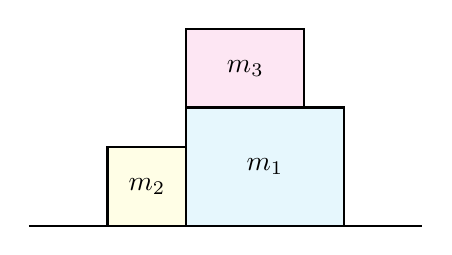
\begin{tikzpicture}[thick]
    \draw (0,0)--(5,0);
    \draw[fill=cyan!10] (2,0) rectangle +(2,1.5) node[midway]{$m_1$};
    \draw[fill=yellow!10] (1,0) rectangle +(1,1) node[midway]{$m_2$};
    \draw[fill=magenta!10] (2,1.5) rectangle +(1.5,1) node[midway]{$m_3$};
  \end{tikzpicture}
  \caption{Many objects will have many normal forces}
  \label{fig:many-normal-forces}
\end{figure}



%\begin{frame}{Normal Forces with Multiple Contact Surfaces}
In Fig.~\ref{fig:normal-force-on-m1}, we see that mass $m_1$ is only in contact
with $m_3$, therefore there is one normal force $\bm F_{n_{31}}$, acting at the
interface between $m_3$ and $m_1$. At this time, we know the \emph{direction}
of $\bm F_{n_{13}}$, but not its \emph{magnitude}, which depends on the motion
of these masses. Finding the magnitude will be part of the analysis process.
\begin{figure}[ht]
  \centering
  \begin{subfigure}{.3\textwidth}
    \centering
    \begin{tikzpicture}[thick,scale=.8]
      \draw (0,0)--(5,0);
      \draw[fill=gray!10] (2,0) rectangle +(2,1.5) node[midway]{$m_3$};
      \draw[fill=gray!10] (1,0) rectangle +(1,1) node[midway]{$m_2$};
      \draw[fill=magenta!10] (2,1.5) rectangle +(1.5,1);
      \draw[ultra thick] (2,1.5)--+(1.5,0);
      \draw[vector] (2.75,2)--+(0,1.3) node[pos=1.15]{$\bm F_{n_{31}}$};
      \fill (2.75,2) circle (.06);
    \end{tikzpicture}
    \caption{Normal force acting on $m_1$ at the interface with $m_3$}
    \label{fig:normal-force-on-m1}
  \end{subfigure}
  \begin{subfigure}{.3\textwidth}
    \centering
    \begin{tikzpicture}[thick,scale=.8]
      \draw (0,0)--(5,0);
      \draw[fill=gray!10] (2,0) rectangle +(2,1.5) node[midway]{$m_3$};
      \draw[fill=yellow!10] (1,0) rectangle +(1,1);
      \draw[fill=gray!10] (2,1.5) rectangle +(1.5,1) node[midway]{$m_1$};
      \draw[ultra thick] (1,0)--+(1,0);
      \draw[vectors] (1.5,.5)--+(0,1.5) node[left]{$\bm F_{n_2}$};
      \draw[ultra thick] (2,0)--+(0,1);
      \draw[vectors] (1.5,.5)--+(-1.5,0) node[left]{$\bm F_{n_{32}}$};
      \fill (1.5,.5) circle (.07);
    \end{tikzpicture}
    \caption{Normal forces acting on $m_2$ at the interface with $m_3$ and
      the bottom surface}
    \label{fig:normal-force-on-m2}
  \end{subfigure}
  \begin{subfigure}{.3\textwidth}
    \centering
    \begin{tikzpicture}[thick,scale=.8]
      \draw (0,0)--(5,0);
      \draw[fill=cyan!10] (2,0) rectangle +(2,1.5);
      \draw[fill=gray!10] (1,0) rectangle +(1,1) node[midway]{$m_2$};
      \draw[fill=gray!10] (2,1.5) rectangle +(1.5,1) node[midway]{$m_1$};
      \draw[ultra thick] (2,1.5)--+(1.5,0);
      \draw[vectors] (3,.75)--+(0,-1.5) node[left]{$\bm F_{n_{13}}$};
      \draw[ultra thick] (2,0)--+(0,1);
      \draw[vectors] (3,.75)--+(1.5,0) node[right]{$\bm F_{n_{23}}$};
      \draw[ultra thick] (2,0)--+(2,0);
      \draw[vectors] (3,.75)--+(0,1.5) node[right]{$\bm F_{n_3}$};
      \fill (3,.75) circle (.07);
    \end{tikzpicture}
    \caption{Normal forces on $m_3$}
    \label{fig:normal-force-on-m3}
  \end{subfigure}  
\end{figure}

In Fig.~\ref{fig:normal-force-on-m2}, mass $m_2$ is in contact with both the
bottom surface as well as with $m_3$, therefore there are \emph{two} normal
forces. Again, we know the \emph{directions} of $\bm F_{n_{12}}$ and
$\bm F_{n_2}$, but not their \emph{magnitudes}.

In Fig.~\ref{fig:normal-force-on-m3}, mass $m_3$ is in contact with $m_2$ and
$m_3$, as well as with the bottom surface. Therefore there are \emph{three}
normal forces. Once again, we know the direction of  $\bm F_{n_{31}}$,
$\bm F_{n_{21}}$ and $\bm F_{n_3}$, but not their \emph{magnitudes}.
%  \item $\bm N_{21}$ and $\bm N_{12}$ (which acts on $m_2$) is an
%    action-reaction pair of forces with equal magnitude and opposite direction
%    (3rd law of motion), and
%  \item $\bm N_{31}$ and $\bm N_{13}$ (which acts on $m_3$) is also an
%    action-reaction pair
%  \end{itemize}
%\end{frame}



%\subsection{Normal Force}
%\begin{figure}[ht]
%  \centering
%  \begin{tikzpicture}
%    \draw[thick] (-1,0)--(2.5,0);
%    \draw[mass] rectangle (1.5,1);
%    \fill (.75,.5) circle (2pt);
%    \draw[vector] (.75,.5)--(.75,-.5) node[below]{$\bm F_g$};
%    \draw[vector] (.75,.5)--(.75,1.5) node[above]{$\bm F_n$};
%  \end{tikzpicture}
%\end{figure}
%
%\begin{itemize}
%\item A force a surface exerts on another object that it is in contact with
%\item Always \textbf{perpendicular} to the contact surface
%\item\textbf{Special case:} When an object is on a horizontal surface
%  with no additional applied force, the magnitude of the normal force is
%  equal to the magnitude of the weight of the object, i.e.\ $N=mg$
%\end{itemize}
%The normal force remains perpendicular to the support surface even when it is
%at an angle:
%\begin{figure}[ht]
%  \centering
%  \begin{tikzpicture}[scale=.9]
%    \draw[thick] (0,0)--(5,0);
%    \draw[axes] (1.7,0) arc (0:30:1.7) node[pos=.6,right] {$\theta$};
%    \begin{scope}[rotate=30]
%      \draw[thick] (0,0)--(5,0);
%      \draw[mass] (2,0) rectangle (4,1.5);
%      \draw[vector,rotate around={-30:(3,.75)}]
%      (3,.75)--(3,-1) node[right]{$\bm F_g$};
%      \draw[vector,red] (3,.75)--(3,2.25) node[left=-1]{$\bm F_N$};
%      \fill (3,.75) circle (.06);
%    \end{scope}
%  \end{tikzpicture}
%\end{figure}
%\textbf{Important note:} It is not always clear what the magnitude of the
%normal force is. Finding the magnitude of the normal force is part of the
%analysis process.




%%\begin{frame}{Normal Force on a Stationary Slope}
%  For this case, we define the $x$-axis to be along the slope, and $y$-axis to
%  be perpendicular to the slope.
%  \begin{columns}
%    \column{.35\textwidth}
%    \centering
%    \begin{tikzpicture}[scale=.9]
%      \draw[thick] (-1,0)--(3,0);
%      \draw[thick,->](.1,0) arc(0:37:1.1) node[pos=0,below]{$\theta$};
%      \begin{scope}[rotate around={37:(-1,0)}]
%        \draw[->](3.5,.5)--(4,.5)  node[right]{$x$};
%        \draw[->](3.5,.5)--(3.5,1) node[above]{$y$};
%        \draw[thick] (-1,0)--(4,0);
%        \draw[fill=cyan!80,thick] rectangle (3,2);
%        \fill(1.5,1) circle (2pt);
%        \draw [->,very thick,dotted,red] (1.5,1)--(1.5,-.5)
%        node[right]{$mg\cos\theta$};
%        \draw [->,very thick,dotted,red] (1.5,1)--(.45,1)
%        node[left]{$mg\sin\theta$};
%        \draw [->,very thick,red] (1.5,1)--(.45,-.5)
%        node[below]{$\bm F_g$};
%        \draw [->,very thick] (1.5,1)--(1.5,2.5) node[above]{$\bm F_N$};
%      \end{scope}
%    \end{tikzpicture}
%    
%    \column{.65\textwidth}
%    \begin{itemize}
%    \item On a stationary slope: $N=mg\cos\theta$
%      \begin{itemize}
%      \item $N$ decreases as ramp angle $\theta$ increases
%      \end{itemize}
%    \item Weight has a component along the ramp ($mg\sin\theta$) that wants
%      to slide the block down.
%    \end{itemize}
%  
%



\subsection{Friction}
\begin{itemize}
\item A force that opposes the sliding of two surface against one another
\item Always act in a direction that opposes motion or attempted motion
\item Depends on:
  \begin{itemize}
  \item Normal force $N$: The force the two surfaces are pressed against
    each other
  \item Coefficients of friction ($\mu_s$ and $\mu_k$): Smoothness of the
    surfaces, which itself depends on
    \begin{itemize}
    \item The material(s) the surfaces are made of
    \item The use of lubricants
    \end{itemize}
  \end{itemize}
\end{itemize}
\begin{center}
  \pic{.5}{dynamics-calculus/graphics/friction}
\end{center}




\subsubsection{Static Friction}
When there is no relative motion between the two surface, the friction is
called the \textbf{static friction}
%  \textbf{Static friction} between the two surfaces is when there is no
%  relative motion between them
\begin{itemize}
\item Increases with increasing applied force
\item Maximum when the object is just about to move
\end{itemize}
\begin{equation}
  \boxed{f_s\leq\mu_sN}
\end{equation}
\begin{center}
  \begin{tabular}{l|c|c}
    \rowcolor{pink}
    \textbf{Quantity} & \textbf{Symbol} & \textbf{SI Unit} \\ \hline
    Magnitude of static friction & $f_s$ & \si\newton \\
    Coefficient of static friction & $\mu_s$ & no units \\
    Magnitude of normal force    & $N$ & \si\newton
  \end{tabular}
\end{center}




\subsubsection{Kinetic Friction}
When the two surfaces are moving relative to each other, the friction is
called \textbf{kinetic friction} $f_k$. $f_k$ is approximately constant along
the path of movement as long  as $\bm F_N$ stays constant
\begin{equation}
  \boxed{f_k = \mu_kN}
\end{equation}
\begin{center}
  \begin{tabular}{l|c|c}
    \rowcolor{pink}
    \textbf{Quantity} & \textbf{Symbol} & \textbf{SI Unit} \\ \hline
    Magnitude of kinetic friction & $f_k$ & \si\newton \\
    Coefficient of kinetic friction & $\mu_k$ & no units \\
    Magnitude of normal force & $N$ & \si\newton
  \end{tabular}
\end{center}




%\begin{frame}{Static and Kinetic Coefficients of Friction}    
Coefficient of kinetic friction is always lower than the coefficient for
static friction, otherwise nothing will ever move:
\begin{equation}
  \mu_k\leq\mu_s
\end{equation}

Consider a simple case of a box being pulled along a level floor. The free-body
diagram is simple (left). How do the magnitudes of the applied force $F_a$ and
friction $f$ compare?

\begin{figure}[ht]
  \centering
  \begin{tikzpicture}
    \draw[thick] (-1,0)--(2.5,0);
    \draw[mass] rectangle (1.5,1);
    \fill (.75,.5) circle (2pt);
    \draw[vector] (.75,.5)--(.75,-.5) node[below]{$\bm F_g$};
    \draw[vector] (.75,.5)--(.75,1.5) node[above]{$\bm F_N$};
    \draw[vector] (.75,.5)--(2.,.5) node[right]{$\bm F_a$};
    \draw[vector] (.75,.5)--(.1,.5) node[left]{$\bm f$};
  \end{tikzpicture}
\end{figure}
%    \column{.6\textwidth}
%    \centering
%    \begin{tikzpicture}[scale=.5,vector]
%      \draw (0,0)--(10,0) node[right]{$F_a$};
%      \draw (0,0)--(0,5) node[left]{$f$};
%    \end{tikzpicture}
  




%\begin{frame}{Tires}
Most people associate friction as the force that slows down things, but very
often friction is what accelerates things. \textbf{Example:} the forward
acceleration of a car is caused by the static friction between the tires and
the road.
\begin{center}
  \pic{.38}{dynamics-calculus/graphics/all-season-tires}
\end{center}
Tires also generated a force called \emph{rolling resistance} as it rolls
along a road because the weight of the car deforms the tires.





\subsection{Drag}
\label{sec:drag}

When an object moves through a fluid (most gases and liquids), it experiences
a fluid resistance force called \textbf{drag} $\bm F_D$. It is defined as:
\begin{important-equation}
    F_D=\frac12\rho v_\infty^2C_DA
\end{important-equation}
Unlike kinetic friction, drag force scales with the square of the speed of the
object relative to the fluid that it is moving in:
\begin{figure}[ht]
  \pic{.338}{dynamics-calculus/graphics/boeing787}
  \pic{.35}{dynamics-calculus/graphics/ganna}
  \pic{.263}{dynamics-calculus/graphics/submarine}
  \caption{Object moving through fluids will experience a drag force}
  \label{fig:drag}
\end{figure}
At this time, you are not required to know the drag equation, just that
$F_D\propto v^2$, and $F_D\propto A$
%\begin{equation}
%  \boxed{
%    F_D=\frac12\rho v_\infty^2C_DA
%  }
%\end{equation}  
%\begin{center}
%  \begin{tabular}{l|c|c}
%    \rowcolor{pink}
%    \textbf{Quantity} & \textbf{Symbol} & \textbf{SI Unit} \\ \hline
%    Magnitude of drag force & $F_D$     & \si\newton \\
%    Density of the fluid    & $\rho$    & \si{\kilo\gram\per\metre\cubed}\\
%    Free-stream velocity    & $v_\infty$ & \si{\metre\per\second}\\
%    Reference area          & $A$       & \si{\metre\squared}\\
%    Drag coefficient        & $C_D$     & (no unit)
%  \end{tabular}
%\end{center}
Drag force also depends on the \textbf{drag coefficient} $C_D$,
a non-dimensional variable that depends on the shape and surface smoothness of
the object.
For blunt objects (``bluff bodies'') $A$ is the frontal area; for
streamlined objects $A$ is the planform (top-view) area.

When we take drag force into account, we understand that the drag force
increases as an object speeds up, and therefore a free-falling object does
\emph{not} accelerate infinitely. Instead it reaches a
\textbf{terminal velocity}.

\begin{figure}[ht]
  \centering
  \begin{subfigure}{.31\textwidth}
    \centering
    \begin{tikzpicture}[scale=.9,vector]
      \draw (0,0)--(0,-1.5) node[below]{$\bm F_g$};
      \draw[black!2] (0,0)--(0,1.5) node[above]{$\bm F_D$};
      \fill circle (.07);
    \end{tikzpicture}    
    \caption{There is no air resistance just as the object \emph{begins}
      to fall. Acceleration is due to gravity alone.}
  \end{subfigure}
  \begin{subfigure}{.31\textwidth}
    \centering
    \begin{tikzpicture}[scale=.9,vector]
      \draw (0,0)--(0,-1.5) node[below]{$\bm F_g$};
      \draw[black!2] (0,0)--(0,1.5) node[above]{$\bm F_D$};
      \draw[green] (0,0)--(0,.6) node[above]{$\bm F_D$};
      \fill circle (.07);
    \end{tikzpicture}
    \caption{Drag increases as $v$ increases. Magnitude of acceleration
      decreases, but the object continues to gather speed}
  \end{subfigure}
  \begin{subfigure}{.31\textwidth}
    \centering
    \begin{tikzpicture}[scale=.9,vector]
      \draw (0,0)--(0,-1.5) node[below]{$\bm F_g$};
      \draw[red] (0,0)--(0,1.5) node[above]{$\bm F_D$};
      \fill circle (.07);
    \end{tikzpicture}
    \caption{Terminal velocity is reached when the drag force equals the
      object's weight. Not net force; no acceleration.}
  \end{subfigure}
\end{figure}



%  \textbf{Example:} To move a \SI{45}{kg} wooden crate across a wooden floor
%  ($\mu=0.20$), you tie a rope onto the crate and pull on the rope. While you
%  are pulling the rope with a force of \SI{115}{N}, it makes an angle of
%  \ang{15}
%  with the horizontal. How much time elapses between the time at which the
%  crate just starts to move and the time at which you are pulling it with a
%  velocity of \SI{1.4}{m/s}?
%  \begin{center}
%    \pic{.5}{dynamics-calculus/graphics/pull-box}
%  \end{center}

%  \textbf{Example:} You are holding an \SI{85}{kg} trunk at the top of a ramp
%  that slopes from a moving van to the ground, making an angle of \ang{35} with
%  the ground. You lose your grip and the trunk begins to slide.
%  \begin{itemize}
%  \item If the coefficient of friction between the trunk and the ramp is
%    $0.42$, what is the acceleration of the trunk?
%  \item If the trunk slides \SI{1.3}{m} before reaching the bottom of the ramp,
%    for what time interval did it slide?
%  \end{itemize}



%  \textbf{Example:} A \SI{55}{kg} person is standing on a scale in an
%  elevator. If
%  the scale is calibrated in \emph{newtons}, what is the reading on the scale
%  when the elevator is not moving? If the elevator begins to accelerate upward
%  at \SI{.75}{m/s^2}, what will be the reading on the scale?




\subsection{Tension Force}
\textbf{Tension} $\bm F_T$ is the force that is transmitted through objects
that can be stretched, e.g.\ a rope that is being pulled
\begin{center}
  \pic{.6}{dynamics-calculus/graphics/3-rope}
\end{center}
\begin{itemize}
\item Examples: ropes, cables, strings, etc.
\item Tension force can only be transmitted if the cable is fully extended
\item You can't push on a rope
\item Can be used with pulleys to change the direction of force
\end{itemize}




\subsection{Spring Force}
The spring force $\bm F_e$ is the force that a compressed/stretched spring
exerts on the object connected to it. An \emph{ideal} spring obeys Hooke's law:
\begin{important-equation}
  \bm F_e=-k\bm x
\end{important-equation}
The spring force acts in the opposite direction to the spring's displacement,
and is proportional to the amount of compression/stretching of the spring
$\bm x$. The proportionality constant $k$ is called the
\textbf{spring constant} (or \textbf{force constant}, or
\textbf{Hooke's constant}, or in many engineering textbooks, the
\textbf{spring rate}), with an SI unit of \emph{newton per metre}
(\si{\newton\per\metre}).
\begin{figure}[ht]
  \centering
  \begin{subfigure}{.47\linewidth}
    \centering
    \begin{tikzpicture}
      \draw[mass] (5,.5) rectangle (6,1.5);
      \draw[thick,
        decoration={aspect=.6,segment length=5mm, amplitude=2.5mm, coil},
        decorate] (0,1)--(5,1);
      \fill[pattern=north east lines] (-.2,0) rectangle (0,2);
      \draw[thick] (0,.0)--(0,2);
      \fill[red] (5.5,1) circle (.06);
      \draw[vector,red] (5.5,1)--(4,1) node[above]{$\bm F_e$};
      \draw[dashed] (3,0)--(3,2) node[above]{unstretched position};
      \draw[vector] (3,.3)--(5,.3) node[midway,below]{$\bm x$};
    \end{tikzpicture}
    \caption{A spring in extension}
  \end{subfigure}
  \begin{subfigure}{.47\linewidth}
    \centering
    \begin{tikzpicture}
      \draw[thick,gray!40,fill=gray!20] (5,.5) rectangle (6,1.5);
      \draw[thick,gray!20,
        decoration={aspect=.6,segment length=5mm, amplitude=2.5mm, coil},
        decorate] (0,1)--(5,1);
      \fill[pattern=north east lines](-.2,0) rectangle (0,2);
      \draw[thick](0,.0)--(0,2);
      \fill[gray!30] (5.5,1) circle (.06);
      \draw[vector,gray!30] (5.5,1)--(4,1) node[above]{$\bm F_e$};
      \draw[dashed](3,0)--(3,2)  node[above]{unstretched position};
      \draw[vector,gray!30](3,.3)--(5,.3)node[midway,below]{$\bm x$};
      \draw[mass] (1.5,.5) rectangle (2.5,1.5);
      \draw[thick,
        decoration={aspect=.3,segment length=1.5mm, amplitude=2.5mm, coil},
        decorate] (0,1)--(1.5,1);
      \draw[vector] (3,.3)--(1.5,.3) node[midway,below]{$\bm x$};
      \fill[red] (2,1) circle (.06);
      \draw[vector,red] (2,1)--(3,1) node[above]{$\bm F_e$};
    \end{tikzpicture}
    \caption{A spring in compression}
  \end{subfigure}
\end{figure}

The spring force is called a \emph{restoring force} because it always points
towards the unstretched position. This restoring nature of the force why the
spring force causes the mass to vibrate. This further discussed in
Chapter~\ref{chapter:harmonic-motion}, on harmonic motion.


\section{Free-Body Diagrams}

Acceleration (if there is going to be any at all) depends on net force
$\bm F_\text{net}$. Without a vector sum of all the forces, we cannot determine
the magnitude, direction of the acceleration, or how acceleration will evolve
in time. To help is visualiz forces acting on an object, we use
\textbf{free-body diagrams} (FBD) to represent all the forces. FBDs are a very
important standard technique when solving any dynamics problems, and is not
a step that should be skipped.

For \emph{rectilinear}, or \emph{translational} motion, FBDs are usually drawn
by assuming that all forces acting at the center of mass (``CM''),
represented by the ``big dot''. For example:
\begin{figure}[ht]
  \centering
  \begin{tikzpicture}[scale=.8]
    \fill (1.5,1) circle (.1);
    \draw[vector] (1.5,1)--(1.5,-.5) node[below]{$\bm F_g$};
    \draw[vector] (1.5,1)--(1.5,2.5) node[above]{$\bm F_N$};
    \draw[vector] (1.5,1)--(3.1,1) node[right]{$\bm F_a$};
    \draw[vector] (1.5,1)--(.75,1) node[left] {$\bm f$};
  \end{tikzpicture}
\end{figure}

However, for motion where \emph{rotation} is (at least) a possibility, we
must note that while gravitational force $\bm F_g$ acts at CM, normal
force $\bm F_N$, friction $\bm f$ and applied force $\bm F_a$ all act at the
point of contact, away from the CM. In those cases, forces should be drawn
where they are applied. For example, a sphere rolling down a ramp should have
weight $\bm F_g$, normal force $\bm F_N$ and static friction $\bm f_s$ acting
on it, as shown in Fig.~\ref{fig:rollingdown1}
\begin{figure}[ht]
  \centering
  \begin{tikzpicture}[scale=1.1,rotate=-30]
    \shade[ball color=red!20] circle (1);
    \draw[thick] (-2,-1)--(2,-1);
    \fill circle (.05);
    \draw[vector,rotate=30] (0,0)--(0,-1.5) node[below]{$\bm F_g$};
    \draw[vector] (0,-1)--(0,.3) node[above]{$\bm F_N$};
    \draw[vector] (0,-1)--(-.5,-1) node[left]{$\bm f_s$};
    \draw[axes] (2,0)--(2.5,0) node[right]{$x$};
    \draw[axes] (2,0)--(2,.5) node[above]{$y$};
    \draw[axes] (0,1.2) arc (90:60:1.2) node[pos=.3,right]{$\omega$};
  \end{tikzpicture}
  \caption{Free-body diagram of a sphere rolling down a ramp without slipping}
  \label{fig:rollingdown1}
\end{figure}

Once the FBD is drawn, decide on the axes to help you solve the motion. One of
the axes should line up with the direction of motion. This guarantees that
the \emph{other} axis will not have any net force.

%\begin{frame}{Example Problem}
A more difficult static problem may involve two surfaces with two different
friction coefficients. For example, a ladder leaning on a wall. This problem
cannot be solved without first understanding rotational motion, but we can
still draw a FBD.

\textbf{Example:} A uniform ladder is \SI{5.0}{\metre} long and weighs
\SI{400}\newton. The ladder rests against a slippery vertical wall, as
shown in the figure. The inclination angle between the ladder and the rough
floor is \ang{53}. Find the reaction forces from the floor and
from the wall on the ladder and the coefficient of static friction $\mu_s$
at the interface of the ladder with the floor that prevents the ladder from
slipping.
\begin{center}
    \pic{.3}{dynamics-calculus/graphics/ladder}
\end{center}




%\section{Multi-Body Problems}
%
%\begin{figure}[ht]
%  \pic1{dynamics-calculus/graphics/worldslongestroadtrainwithpowertrailer8}
%  \caption{A road train that is common in Australia}
%  \label{fig:roadtrain}
%\end{figure}
%\begin{itemize}
%\item The objects are connected by a cable or a solid linkage with negligible
%  mass
%\item All objects (usually) have the same acceleration
%\item Require multiple free-body diagrams
%\end{itemize}
%
%
%
%To solve a connected-bodies problem, you can follow these procedures:
%\begin{enumerate}
%\item Draw a FBD on each of the objects
%\item Sum all the forces on all the objects along the direction of motion
%  \begin{itemize}
%  \item Direction of motion is usually very obvious
%  \item All internal forces should cancel and do not figure into the
%    acceleration of the system
%  \end{itemize}
%\item Compute the acceleration of the entire system using second law of motion
%  \begin{itemize}
%  \item Remember that (usually) every object has the same acceleration!
%  \end{itemize}
%\item Go back to the FBD of each of the objects and compute the unknown
%  forces (usually tension)
%\end{enumerate}
%
%
%
%%  \textbf{Example:} A tractor-trailer pulling two trailers starts from rest
%%  and accelerates with an acceleration $a$ on a straight, level road. The mass
%%  of the truck (T) is \SI{5450}{\kilo\gram}, the mass of the first trailer (A)
%%  is \SI{31500}{\kilo\gram}, and the mass of the second trailer (B) is
%%  \SI{19600}{\kilo\gram}.
%%  \begin{enumerate}
%%  \item What magnitude of force must the truck generate in order to accelerate
%%    the entire vehicle?
%%  \item What magnitude of force must each of the trailer hitches withstand
%%    while the vehicle is accelerating?
%%  \end{enumerate}
%%  Assume that frictional forces are negligible in comparison with the forces
%%  needed to accelerate the large masses.
%%
%
%
%
%%\begin{frame}{Different Types of Connected Bodies}
%Multiple objects pressed against one another. There may not be friction, but
%there are definitely action/reaction forces between the blocks.
%\begin{center}
%  \begin{tikzpicture}[scale=.8]
%    \draw[thick] (-3,0)--(4,0);
%    \draw[thick] rectangle (1,1) node[midway]{$m$};
%    \draw[thick] (1,0) rectangle (3,1.5) node[midway]{$M$};
%    \draw[vector] (-1.5,.5)--(0,.5) node[pos=0,left]{$\bm F_a$};
%  \end{tikzpicture}
%\end{center}
%Or multiple objects stacked on top of one another. The contact surface between
%$M$ and the floor may (or may not) have friction, while the surface between
%$M$ and $m$ must have a friction coefficient $\mu$.
%\begin{center}
%  \begin{tikzpicture}[scale=.8]
%    \draw[thick] (-1,0)--(5.5,0);
%    \draw[thick] rectangle (3,1.5) node[midway]{$M$};
%    \draw[thick] (.75,1.5) rectangle (2.25,2.5) node[midway]{$m$};
%    \draw[vector] (3,.5)--(4.5,.5) node[right]{$\bm F_a$};
%  \end{tikzpicture}
%\end{center}
%
%
%
%
%\subsection{Pulley Problems}
%
%\begin{figure}[ht]
%  \centering
%  \begin{tikzpicture}[scale=.7]
%    \draw[ultra thick,brown] (-1,-1.6)--(-1,0);
%    \draw[ultra thick,brown] (1,0)--(1,-3);
%    \draw[thick,fill=gray] circle (1.05);
%    \draw[thick,fill=gray!40] circle (.95);
%    \draw[line width=5.5] (0,-.15)--(0,2);
%    \draw[very thick] (-2,2)--(2,2);
%    \fill[white] circle (.1);
%    \draw[mass] (-1.5,-1.6) rectangle +(1,-1) node[midway]{$M$};
%    \draw[mass] (.5,-3) rectangle +(1,-1.4) node[midway]{$m$};
%  \end{tikzpicture}   
%\end{figure}
%
%An \textbf{Atwood machine} is made of two objects connected by a rope that
%runs over a pulley. The pulley allows the direction of force and direction
%of motion to change between two objects.
%    
%\textbf{Example:} The object on the left has a mass of $M$ and the object on
%the right has a mass of $m$.
%\begin{enumerate}
%\item What is the acceleration of the masses?
%\item What is the tension in the rope?
%\end{enumerate}
%  
%
%%%\begin{frame}{Example Problem: Atwood Machine}
%%  An \textbf{Atwood machine} is made of two objects connected by a rope that
%%  runs over a pulley. The pulley allows the direction of force and direction
%%  of motion to change between two objects.
%%  \begin{columns}
%%    \column{.35\textwidth}
%%    \centering
%%    \pic1{dynamics-calculus/graphics/pulley_prob_2}
%%
%%    \column{.65\textwidth}
%%    \textbf{Example:} The object on the left has a mass of $M$ and the object
%%    on the right has a mass of $m$.
%%    \begin{itemize}
%%    \item What is the acceleration of the masses?
%%    \item What is the tension in the rope?
%%    \end{itemize}
%%  
%%
%
%
%
%%%\begin{frame}{A Difficult Problem!}
%%  \begin{columns}
%%    \column{.6\textwidth}
%%    \textbf{Example:} Two blocks of mass $m$ and $M$ are connected via pulley
%%    with a configuration as shown on the right. The coefficient of static
%%    friction between the left block and the surface is $\mu_{s,1}$, and the
%%    coefficient of static friction between the right block and the surface is
%%    $\mu_{s,2}$. Formulate a mathematical inequality for the condition that no
%%    sliding occurs. There may be more than one inequality. 
%%    
%%    \column{.4\textwidth}
%%    \pic{1}{dynamics-calculus/graphics/pulley_prob_6}
%%  
%%
%%
%%
%%
%%%\begin{frame}{Multiple Pulleys}
%%  When there are multiple pulleys involved, we have to remember that tension
%%  force is distributed evenly along the cable.
%%
%%  \vspace{.2in}
%%  \begin{columns}
%%    \column{.6\textwidth}
%%    \textbf{Example:} A block of mass $m$ is pulled, via two pulleys as shown,
%%    at constant velocity along a surface inclined at angle $\theta$. The
%%    coefficient of kinetic friction is $\mu_k$, between block and surface.
%%    Determine the pulling force $F$. Ignore the mass of the pulleys. 
%%    
%%    \column{.4\textwidth}
%%    \pic{1}{dynamics-calculus/graphics/pulley_prob_7}
%%    
%%
%
%
%%%\begin{frame}{One More!}
%%  \begin{columns}
%%    \column{.75\textwidth}
%%    \textbf{Example:} A block of mass $M$ is lifted at constant velocity, via
%%    an arrangement of pulleys as shown. Determine the pulling force $F$. Ignore
%%    the mass of the pulleys. 
%%
%%    \uncover<2>{
%%      \vspace{.2in}\textbf{Example:} The pulling force is replaced by a $10M$
%%      mass, and was let go. What are the accelerations of the $M$ and the
%%      $10M$ mass?
%%    }
%%    
%%    \pic{1}{dynamics-calculus/graphics/pulley_prob_9}
%%  
%%
%
%
%%\begin{frame}{A More Typical Problem}
%More typically, an Atwood machine problem is one where two objects are
%sliding on a surface. These surfaces may have (or may not) have friction. In
%this example, two blocks are connected by a massless string over a
%frictionless pulley as shown in the diagram.
%\begin{figure}[ht]
%  \centering
%  \begin{tikzpicture}[scale=1.2]
%    \draw[thick,brown] (-4,.4)--(.1,.4);
%      \draw[thick] (0,0)--(-5.5,0) node[midway,below]{$\mu$};
%      \draw[thick,fill=magenta!20] (-4,0) rectangle (-5,.75) node[midway]{$m$};
%      \begin{scope}[rotate=-30,thick]
%        \draw[brown] (1,.4)--(-.05,.4);
%        \draw (0,0)--(3,0) node[midway,below left]{$\mu$};
%        \draw[mass] (1,0) rectangle (2.5,1) node[midway]{$M$};
%      \end{scope}
%      \begin{scope}[rotate=-15]
%        \draw[thick,fill=gray] (0,.3) circle (.15);
%        \draw[thick,fill=lightgray] (0,.3) circle (.1);
%        \draw[ultra thick] (0,0)--(0,.3);
%        \fill (0,.3) circle (.04);
%      \end{scope}
%      \draw[thick,gray!70] (0,0)--(0,-1.5);
%      \draw[axes] (0,-.5) arc (270:330:.5) node[midway,below]{$\phi$};
%  \end{tikzpicture}
%\end{figure}
%\begin{enumerate}
%\item Determine the acceleration of the blocks.
%\item Calculate the tension in the string.
%\end{enumerate}
%
